\begin{frame}
    \frametitle{\problemtitle}
    \begin{itemize}
        \item<+-> \textbf{Problem:} Copy $n$ psalms in at most $2n\sqrt n$ pageflips.
        \item<+-> Most naive solutions use $\mathcal{O}(n^2)$ pageflips, so you need to be smarter.
        \item<+-> Idea: each psalm corresponds to a point in 2D space, and the pageflips needed to copy one psalm after another corresponds to their Manhattan distance.
        \item<+-> So, you need to find a path of bounded length that visits all points.
    \end{itemize}
    \vfill
    \centering
    \onslide<3->
    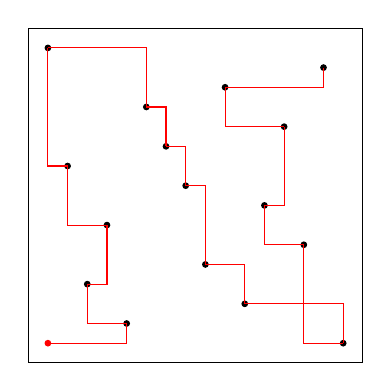
\begin{tikzpicture}
        \draw (-0.25,-0.25) rectangle (4,4);
        \def\psalms{{15,9,3,6,1,12,10,8,4,13,2,7,11,5,14,0}}
        \def\orderopt{{4,2,3,1,0,5,6,7,8,10,15,13,11,12,9,14}}

        \filldraw[red] (0,0) circle[radius=1pt];
        \foreach \i in {0,1,...,15}
            \filldraw[black] (\i/4,\psalms[\i]/4) circle[radius=1pt];

        \onslide<4->{
        \draw[red] (0,0) -- (\orderopt[0]/4,0) -- (\orderopt[0]/4,\psalms[\orderopt[0]]/4);
        \foreach \i in {0,1,...,14}
            \draw[red] (\orderopt[\i]/4,\psalms[\orderopt[\i]]/4) -- (\orderopt[\i+1]/4,\psalms[\orderopt[\i]]/4) -- (\orderopt[\i+1]/4,\psalms[\orderopt[\i+1]]/4);
        }
    \end{tikzpicture}
\end{frame}
\begin{frame}
    \frametitle{\problemtitle}
    \begin{itemize}
        \item \textbf{Problem:} Copy $n$ psalms in at most $2n\sqrt n$ pageflips.
        \item<+-> Solution idea: divide the plane into $\sqrt n$ bands of height $\sqrt n$.
        \item<+-> For the first band, iterate over all points in it from left to right.
        \item<+-> For the second band, iterate over all points from right to left.
        \item<+-> And so on...
    \end{itemize}
    \vfill
    \centering
    \begin{tikzpicture}
        \draw (-0.25,-0.25) rectangle (4,4);
        \def\psalms{{15,9,3,6,1,12,10,8,4,13,2,7,11,5,14,0}}
        \def\orderopt{{2,4,10,15,13,11,8,3,1,6,7,12,14,9,5,0}}

        \foreach \i in {0,1,...,3}
            \filldraw[lightgray] (-0.1,\i-0.1) rectangle (3.85,\i+0.85);

        \filldraw[red] (0,0) circle[radius=1pt];
        \foreach \i in {0,1,...,15}
            \filldraw[black] (\i/4,\psalms[\i]/4) circle[radius=1pt];

        \onslide<2->
        \draw[red] (0,0) -- (\orderopt[0]/4,0) -- (\orderopt[0]/4,\psalms[\orderopt[0]]/4);
        \only<2>{
        \foreach \i in {0,1,...,2}
            \draw[red] (\orderopt[\i]/4,\psalms[\orderopt[\i]]/4) -- (\orderopt[\i+1]/4,\psalms[\orderopt[\i]]/4) -- (\orderopt[\i+1]/4,\psalms[\orderopt[\i+1]]/4);
        }
        \only<3>{
        \foreach \i in {0,1,...,6}
            \draw[red] (\orderopt[\i]/4,\psalms[\orderopt[\i]]/4) -- (\orderopt[\i+1]/4,\psalms[\orderopt[\i]]/4) -- (\orderopt[\i+1]/4,\psalms[\orderopt[\i+1]]/4);
        }
        \onslide<4->{
        \foreach \i in {0,1,...,14}
            \draw[red] (\orderopt[\i]/4,\psalms[\orderopt[\i]]/4) -- (\orderopt[\i+1]/4,\psalms[\orderopt[\i]]/4) -- (\orderopt[\i+1]/4,\psalms[\orderopt[\i+1]]/4);
        }
    \end{tikzpicture}
\end{frame}
\begin{frame}
    \frametitle{\problemtitle}
    \begin{itemize}
        \item \textbf{Problem:} Copy $n$ psalms in at most $2n\sqrt n$ pageflips.
        \item<+-> Each band uses $n$ page flips for the horizontal segments, and at most $1 + 2 + \ldots + \sqrt n \approx n/2$ page flips for the vertical segments.
        \item<+-> The transitions between bands use at most $2n$ page flips total.
        \item<+-> Overall: this uses at most $\sqrt n (n + n/2) + 2n = 1.5n\sqrt n + 2n$ page flips.
    \end{itemize}
    \vfill
    \centering
    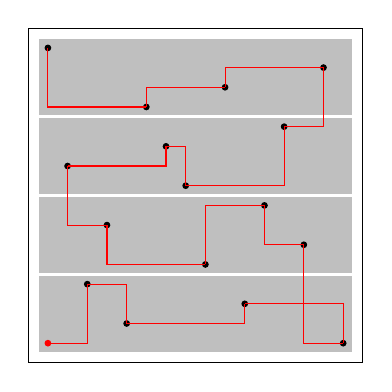
\begin{tikzpicture}
        \draw (-0.25,-0.25) rectangle (4,4);
        \def\psalms{{15,9,3,6,1,12,10,8,4,13,2,7,11,5,14,0}}
        \def\orderopt{{2,4,10,15,13,11,8,3,1,6,7,12,14,9,5,0}}

        \foreach \i in {0,1,...,3}
            \filldraw[lightgray] (-0.1,\i-0.1) rectangle (3.85,\i+0.85);

        \filldraw[red] (0,0) circle[radius=1pt];
        \foreach \i in {0,1,...,15}
            \filldraw[black] (\i/4,\psalms[\i]/4) circle[radius=1pt];

        \draw[red] (0,0) -- (\orderopt[0]/4,0) -- (\orderopt[0]/4,\psalms[\orderopt[0]]/4);
        \foreach \i in {0,1,...,14}
            \draw[red] (\orderopt[\i]/4,\psalms[\orderopt[\i]]/4) -- (\orderopt[\i+1]/4,\psalms[\orderopt[\i]]/4) -- (\orderopt[\i+1]/4,\psalms[\orderopt[\i+1]]/4);
    \end{tikzpicture}
\end{frame}
\begin{frame}
    \frametitle{\problemtitle}
    \begin{itemize}
        \item \textbf{Problem:} Copy $n$ psalms in at most $2n\sqrt n$ pageflips.
        \item<+-> Alternative solution: just greedily go to the nearest unvisited point.
    \end{itemize}
    \vfill
    \begin{center}
    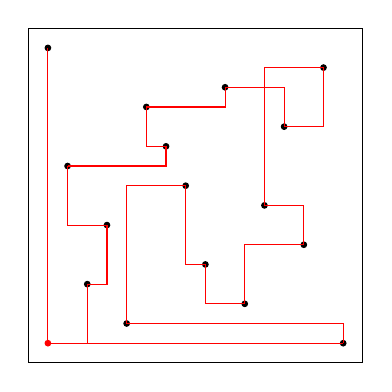
\begin{tikzpicture}
        \draw (-0.25,-0.25) rectangle (4,4);
        \def\psalms{{15,9,3,6,1,12,10,8,4,13,2,7,11,5,14,0}}
        \def\orderopt{{2,3,1,6,5,9,12,14,11,13,10,8,7,4,15,0}}

        \filldraw[red] (0,0) circle[radius=1pt];
        \foreach \i in {0,1,...,15}
            \filldraw[black] (\i/4,\psalms[\i]/4) circle[radius=1pt];

        \draw[red] (0,0) -- (\orderopt[0]/4,0) -- (\orderopt[0]/4,\psalms[\orderopt[0]]/4);
        \foreach \i in {0,1,...,14}
            \draw[red] (\orderopt[\i]/4,\psalms[\orderopt[\i]]/4) -- (\orderopt[\i+1]/4,\psalms[\orderopt[\i]]/4) -- (\orderopt[\i+1]/4,\psalms[\orderopt[\i+1]]/4);
    \end{tikzpicture}
    \end{center}
    \solvestats
\end{frame}
